% Chapter 1

\chapter{Preliminaries}\label{ch:Basis}

\begin{figure}[t]
    \centering
    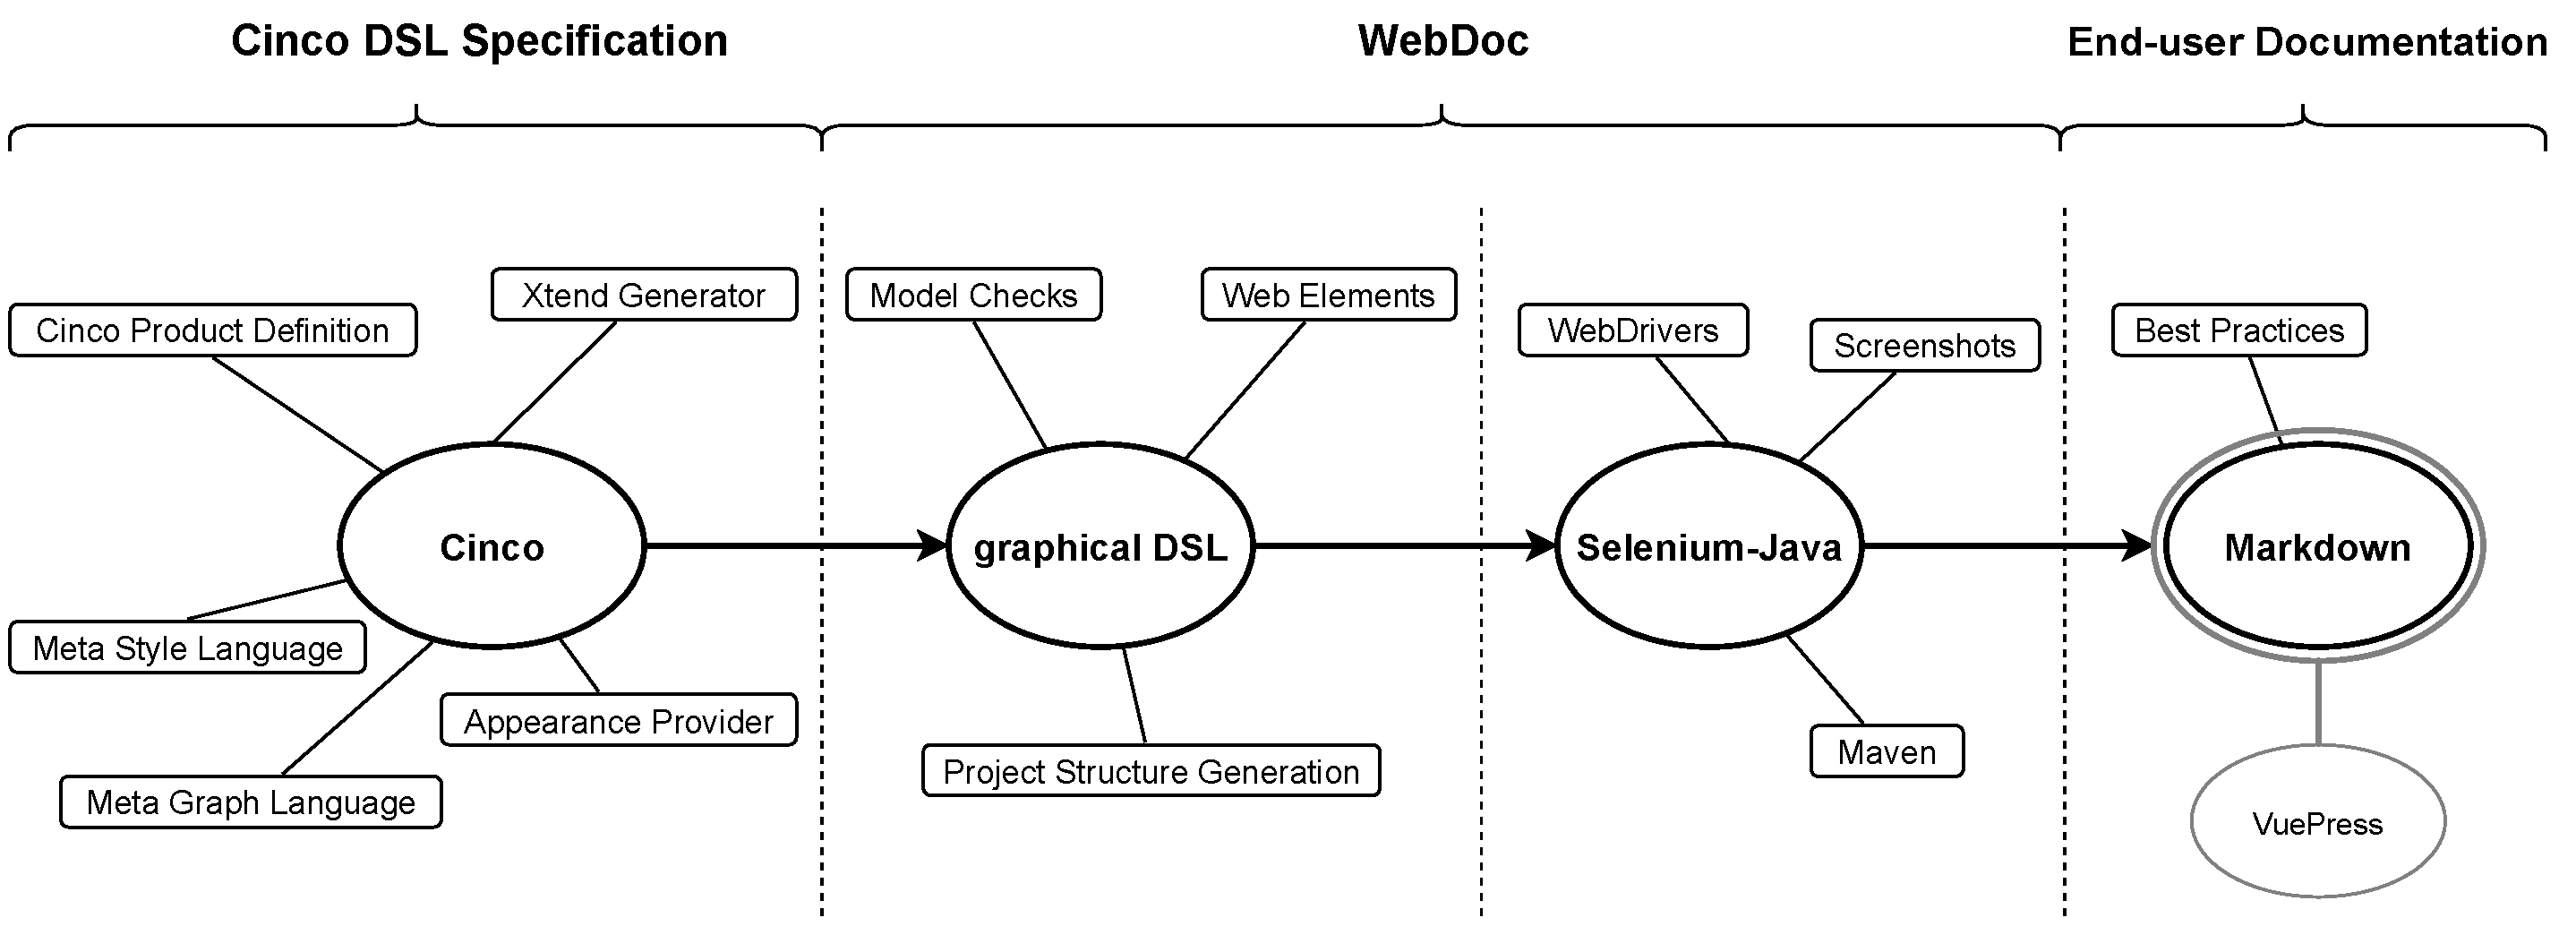
\includegraphics[width=\textwidth]{WebDocDevelopment-all.pdf}
    \caption{Development path of the end user documentation}
    \label{fig:procWorkflow}
\end{figure}

This chapter introduces the key concepts that are required to achieve our goal. We begin by considering the format of our end-user documentation as required by known standards, as well as the technologies available to assist us in completing this task. The \textsc{Cinco} Meta Tooling Suite will next be used to introduce the principles of model-driven programming, as well as introduce the meta languages on which our graphical models are based and quickly describe what needs to be generated from those models. The steps to achieving our aim are depicted in Figure \ref{fig:procWorkflow}.

\pagebreak

\section{End User Documentation}\label{sec:endUserDoc}

The value of a good software product, in fact, of any product destined to be brought to the consumer is determined on how effective the end user can learn to use the product. Hence, putting a great effort to generate and manage a useful, well-structured documentation is as much important as the development of the product itself~\cite{ISO-IEC-IEEE}. 

The goal of end user documentation is to provide application end users with the knowledge they need to interact with the software properly. It is an integral aspect of the development process and serves as a link between the product creator and the end user~\cite{9238529}. By increasing the structure and usability of the information supplied to end users, the developer not only reduces the number of support calls, but also improves the product's and the company's reputation~\cite{ieee5712775}.

In this section we will go through the main characteristics of end user documentation, focusing on the standards establish by the ISO/IEC and the IEEE~\cite{ieee5712775, ISO-IEC-IEEE}. Next, we will talk about the specifics of documenting Web application by giving an example of a documented Web application. We will also present the currently used technologies for creating and managing such documentation. Our main goal is to produce an entire end user documentation page from a graphical model. Before going further, we ought to precise that the type of documentation to be created will depend on how the documentation designer lays out the model, that means the model could be designed to represent a technical documentation -- requiring deep knowledge of the application documented -- or it could also be structured to produce a documentation for simple end users with no technical knowledge at all of the underlying Web application~\cite{ieee6081814}.


\subsection{Documentation Characteristics}\label{sec:char}

Since our focus is primarily on Web applications, we will be documenting the \glsentryfull{ui}, which is composed of Web elements (like buttons, navigation links, checkboxes, etc.) the user can interact with. This settles implicitly the type of documentation we aim to create: a step-by-step guide for navigating UI to reach the expected result. Nonetheless, the ISO/IEC/IEEE Standard 26511:2012~\cite{ieee6170926} mandates i.e.,~that completeness and accuracy should be of the utmost importance when designing the end user documentation.

Bearing that in mind, a good documentation should respond to three important questions: \textit{why} the application has been programmed, meaning the problem the application intends to solve, \textit{what} is the end user supposed to do to get to the solution quickly and efficiently and \textit{how} it is achieved~\cite{ISO-IEC-IEEE}. This is a task we leave to the information manager. The last question, however, is better answered by providing visual help in form of screen captures or any illustration that fastens the understanding of the documentation. 

We plan to document Web applications from the perspective of the application's end user, as previously stated. This means that the documentation developer must consider the product's audience, and identifying the core jobs and activities of common users should be an important element of the design process~\cite{ISO-IEC-IEEE}. The developer is in command of how extensive the documentation becomes using our solution.

\subsection{Documentation Software Tools}

Choosing the format in which the documentation is brought to the end user is as much important as the rest of the milestones of the planning process. A poor decision in this area might limit the documentation's ability to reach a large number of consumers, rendering it useless. Choosing technologies that have already received widespread adoption is a wise move. This ensures a wider reach and prior knowledge within the same audience:

\subsubsection{Markdown}\label{sec:MD}

Markdown is a lightweight markup language created by John Gruber\footnote{John Gruber's official project website \url{https://daringfireball.net/projects/Markdown/}} in 2004. Since, it has established itself as one of the world's most popular markup language~\cite{Markdown}. Gruber states on his webpage that Markdown is comprised of formatting syntaxes that can be applied to plain-text file and optionally a converter to other markup languages files like \gls{html}. In this acronym, Hypertext means the link that connects Web pages to each other, either within the same website or between different websites~\cite{mozillaMDN}. On Mozilla Developer Network website\footnote{MDN: \url{https://developer.mozilla.org/en-US/docs/Web/HTML}}, \gls*{html} is described as the fundamental building block of any Web page, that uses markup syntax to annotate text, images, and other content for display in a Web browser.

For its popularity, it is a great choice for our project, since description of the UI is first made as plain-text and then transform to a rich-text format using markup syntax as depicted below. Moreover, Markdown files can be opened and edited with any kind of text editor available. There is tremendous amount of documentation about Markdown syntax available online for the interested reader to get started.

\begin{figure}[h]
    \centering
    \includegraphics[width=\textwidth]{Markdown.pdf}
    \caption{Plain-text transformation with Markdown}
    \label{fig:Markdown}
\end{figure}

Although there exists a plethora of applications that transform Markdown files into HTML files to be rendered in a Web browser application (i.e. MacDown~\footnote[1]{MacDowns: \url{https://macdown.uranusjr.com/}} for Mac users, ghostwriter~\footnote[2]{Ghostwriters: \url{https://wereturtle.github.io/ghostwriter/}} for Windows and Linux or online tool like Dillinger~\footnote[3]{Dillinger : \url{https://dillinger.io/}}), we choose to work with one framework that also established itself throughout the developer community and that especially works very well with Markdown files: VuePress.

\subsubsection{VuePress}\label{sec:VP}

VuePress is a minimalistic VueJS-powered static website generator. VueJS~\cite{vuepress} is an open source JavaScript framework designed by Evan You\footnote[4]{Eva You's website \url{https://evanyou.me/}}. It is called minimalistic because it only takes a few lines of configuration and two commands to create and launch a static website. It is resilient and up-to-date since it is open source software and is maintained by a large community of contributors.

By respecting the VuePress conventional folder structure, it can explore folders, get Markdown files, and convert them to HTML files. The default appearance of the generated website is defined by a customizable configuration file included in the project folders. By simply adding certain configuration elements, you may create i.e.~a sidebar menu and a navigation bar. VuePress produces a static website by building hyperlinks between HTML files in the project folder hierarchy in the order in which they appear. This means that subfolder Markdown (or HTML) files are rendered as menu items on the folder's HTML page. A server-rendered website with a live reload mechanism is constructed and launched after inputting the correct command. Every modification to the Markdown files is immediately visible on the website. The final step is to create the website, which will be saved in a special folder and can subsequently be exported to any other website.

We will use VuePress to statically launch the end user documentation as a website, relieving the developer of the task of configuring the server. The principal task remaining is therefore to create a solid documentation model.

\section{Core Principles of Model-Driven Development}


This section lays down the fundamentals of the \gls{mdd} -- also referred to as \gls{mdsd}~\cite{fowler} --  using the \textsc{Cinco} SCCE Meta Tooling Framework, as well as the steps necessary to get up and running with the framework. The term MDD refers to a development paradigm where the functionalities of the software are first specified as models, from which then executable code can be automatically generated. To create and use models to represent the software system, a DSL that is close to the problem domain, is needed. Application domain experts possess the knowledge of the application structure, which they represent in form of models. Domain experts and application programmers must agree on how the specification language determines syntax and semantic of the model elements.

The core principles of MDD reside in the fact that software development is accelerated by providing a simple, but efficient abstraction of the software structure as a model. Those model abstraction, representation of real-world objects, are transposed through a series of model-to-model or model-to-code transformations~\cite{stahl_et_al}. Our work is to utilize the DSL provide by the \textsc{Cinco} framework to design our graphical DSL, which in turn will permit the generation of a functioning \gls*{selenium}-Java application (Selenium is a suite of application tools for automating Web browsers) to take screenshots of the different Web application states.

Opposed to the common development method, applying a graphical model to layout the different user sequences allows even non-programmer (here the domain expert with much more expertise on how to design a great software documentation) to accomplish the task of documenting the features offered by the Web application. Nonetheless, the programmer has the tasks -- in collaboration with the domain expert -- to specify the meaning of each model element for the code generation process. 

When applied correctly, the result of the model-driven development process is a tailored application to domain. This reflects one of the main advantages of MDD: the accuracy of directly targeting the specific problem~\cite{brambilla2017model}. Besides, it is still possible to change the DSL so that it adapts to the new challenges emerging during the development process. This can be iterated until the specification reaches preciseness wanted to solve the problem.

\section{Domain Specific Language}\label{sec:DSL}

A \glsentryfull{dsl}, as mentioned before, is a language adapted to specific development domain. In~\cite{Naujokat2018} a succinct analogy to \glsplural*{dsl} is given by saying that it is comparable to a tool specially crafted only for one specific task as opposed to general programming languages, which can be seen as tools for multiple different tasks. If we stick to this analogy, just as one would start with a blueprint to construction a mechanical tool, designing as DSL required similar steps. One must conceptually lay out the behavior and eventually -- in case it is a graphical language we seek to design -- the look of each element that can be used in our DSL.

Blueprinting our DSL is equivalent to defining a metalanguage or meta-DSL to our language. \textit{Meta} literally means \textit{situated behind or beyond}\cite{merriam}. So, metalanguage is a descriptive language that comes before our language and describes the meaning (semantic) and relationship between the objects of our target language. To put it another way, the meta-DSL is the abstract syntax, and the DSL concrete syntax is the result. It is feasible to work our way up the meta-definition modeling hierarchy until we reach a self-referencing language, like it is the case \gls{uml}.

In our case, we want a graphical language for creating models that represent the different parts of a Web application and how the end user can possibly interact with them. The metalanguage to our graphical DSL is provided by the \textsc{Cinco} SCCE Meta Tooling Suite. It comprises the \gls{mgl}, the \gls{msl} and the \gls{cpd}. All have been constructed using Xtext~\cite{bettini2016implementing}, a language Workbench for writing textual \glspl*{dsl}~\cite{naujokat-diss}. The next section explains those concepts in detail.

\section{\textsc{Cinco SCCE} Meta Tooling Framework}\label{sec:cincoFW}


The \textsc{Cinco} Framework is a generator-driven development environment for domain-specific graphical modeling tools~\cite{Cinco}. It is actually developed by the chair of programming systems at the Technical University of Dortmund and one of the many projects of the SCCE Group \footnote[1]{\url{https://www.scce.info/}}, which aims at allowing the application-domain experts, rather than programming experts, to take charge of the development tasks~\cite{scce}. One of the great features of this framework is that it allows us to generate an entire editor application with just one click from a simple textual specification language -- the MGL mentioned in the previous section. 

The MGL together with the MSL form the metamodel from which \textsc{Cinco} generates a ready-to-run modeling tools called \textsc{Cinco} product. The MSL is where the \textsc{Cinco} developer defines the look every node and edge element, as well as the font and color of the text to be displayed in the graphical model~\cite{naujokat-diss}. The created metamodel is based on Ecore, the metamodeling language of the \gls{emf} and the Graphiti framework is used to generate the corresponding graphical model editor. Additionally, you find the right button to trigger code generation in the created editor. Chapter~\ref{ch:CP} is devoted to our \textsc{Cinco} product (the editor application), in particular section~\ref{sec:GenProcess} gives an in-depth explanation of the generation process.

\begin{figure}[h]
    \centering
    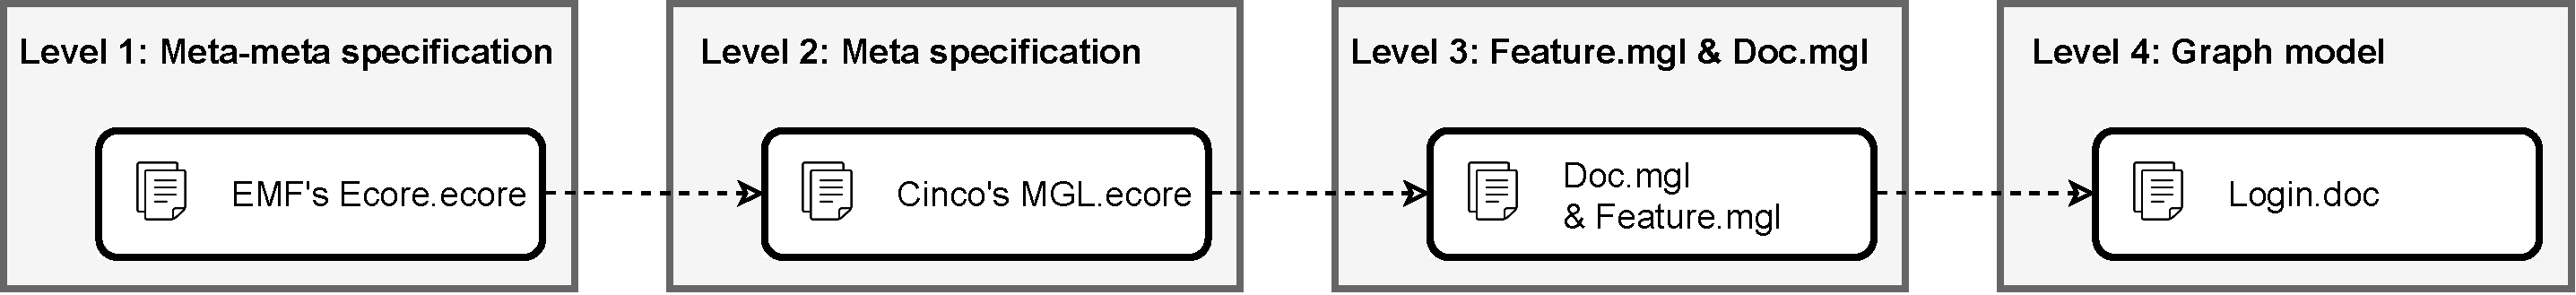
\includegraphics[width=\textwidth]{SpecsHierarchy.pdf}
    \caption{Hierarchy of our graphical DSL specification}
    \label{fig:modeling-hierachy}
\end{figure}

The full generation process of a graphical modeling tool (of a \textsc{Cinco} Product Application) comprises four essential (meta) levels~\cite{Naujokat2018}. The first level, associated with the role Eclipse Developer, is where the Ecore.ecore and GraphitiDiagram.ecore metamodel are developed. The second level is where \textsc{Cinco} Developers of the Chair 5 for Programming Systems used the metamodel from the first level to develop the MGL.ecore, which in turn becomes metamodel of the third specification level, where the \textsc{Cinco} Product Developer operates and where this thesis comes in, see fig.~\ref{fig:modeling-hierachy}. This means the Eclipse Developers are now at the meta-metalevel, the \textsc{Cinco} Developers at metalevel of the specification elaborated in this work. For the remainder of the chapters we will be focusing on the third and fourth specification level. Latter is the level where the \textsc{Cinco} Product Users use the generated graphical editor to create the domain specific models.

\subsection{Meta Graph Language}\label{sec:MGL}

The \gls*{mgl} sketches the behavior, the constraints and gathers the all the graphical components that will constitute the model elements that come in use in every graph diagram created in the modeling tool. This is where we start developing our editor application: the main elements that can be define in a MGL are \textbf{nodes}, \textbf{containers} and \textbf{edges} as illustrates listing~\ref{featMGL}.

The main graph model, the \lstinline{FeatureGraphModel}, is the one containing all the features of the Web application we want documented. For instance, our  Web application provides the login feature as starting point, then after successfully logging in and getting access to the dashboard, task lists can be created or deleted, tasks can be added to or removed from them, etc. The graph diagram can be assigned name and description. We specified \lstinline{.feat} (short for feature) as model extension. And since the login feature i.e.,~requires a series of user actions to be performed, the FeatureGraphModel contains another graph model type, where those sequences of actions will be modeled: the \lstinline{DocGraphModel}. It contains the meta specification of all the commonly used Web elements (i.e., input field, buttons, dropdown, etc.) we want to use in our graph models, as well as sectioning elements to structure the diagram and edges to connect them to each other. The listing below shows an excerpt from the concrete FeatureGraphModel implementation.

\begin{lstlisting}[language=MGL, caption={Excerpt from the feature.mgl, meta-specification of the FeatureGraphModel}, label=docMGL, escapechar=|]
    graphModel FeatureGraphModel { |\label{line:modelStart}|
        iconPath "icons/16/feature_16.png"
        diagramExtension "feat"
        containableElements(FeatureContainer,DocNode[1,*])
        attr EString as modelName := "New Feature"
        attr EString as description := "New Description"
    }|\label{line:modelEnd}|
    
    container FeatureContainer { |\label{line:featCont}|
        style featureContainer("${title}")
        containableElements(Start[1,1], Stop[1,1],DocNode[1,*])
        attr EString as title := "New Feature"
        @multiLine
        attr EString as documentation := "This feature is about ..."
    }
    
    node DocNode{ |\label{line:docNode}|
        style docNode("${mgl.modelName}")
        prime docMgl::DocGraphModel as mgl |\label{line:prime}|
        attr EBoolean as createScreenshots := true
        incomingEdges (Edge[1,1])
        outgoingEdges (Edge[1,1])
    }
\end{lstlisting}

As you can see we define a container element to hold the DocGraphModel instances (see lines~\ref{line:featCont} and \ref{line:docNode}). To integrate a whole DocGraphModel inside a FeatureGraphModel we used the so called \textit{PrimeReference}, which is a \textsc{Cinco} feature that allows to reference another model by only one attribute of a node or container~\cite{Cinco}. It is applied by adding the keyword \lstinline[language=MGL]{prime}, as we did in line~~\ref{line:featCont}. By doing so, we can simply drag and drop a DocGraphModel diagram into a FeatureGraphModel diagram to incorporate it.

As for the DocGraphModel, we specified four categories of model elements to use while designing the diagram: the most important ones, the Web elements, represent the UI element the user can interact with. The we have the Selenium action nodes, which perform some actions to drive the Web browser through the Selenium WebDriver. This are i.e.,~the Navigation node to change from one Web page to another and the Screenshot node to capture the application current state as an image. Finally, we have the semantic element \lstinline{Comment}, to give a descriptive text to the screenshots and the basic elements (start and end as well as the section node) which help structure the user sequence graph.

\begin{lstlisting}[language=MGL, caption={Excerpt from the Doc.mgl, meta-specification of the DocGraphModel}, label=featMGL, escapechar=|]
    graphModel DocGraphModel {
        iconPath "icons/16/sequence_16.png"
        diagramExtension "doc"
        containableElements(*)
        attr EString as modelName := "UserSequence"
        @multiLine
        attr EString as documenation := "Lorem ipsum dolor et si met"
    }
    
    node Screenshot {
        style screenshotNode
        incomingEdges (Transition[1,1], Anchor[1,*])
        outgoingEdges (Transition[1,*])
        attr EString as pictureName
        attr Comment as description
    }

    node Input extends WebElement {
        style inputNode("Input: ${content}")
        attr EString as content
        incomingEdges (Transition[0,*])
        outgoingEdges (Transition[0,*])
    }
\end{lstlisting}

For demonstration purposes, we kept our example listings short. An exhaustive list of all the usable elements and annotations can be found on the \textsc{Cinco}'s documentation page\footnote[1]{Wiki page : \url{https://gitlab.com/scce/cinco/-/wikis/Cinco-Product-Specification}}.

\subsection{Meta Style Language}\label{sec:MSL}

The appearance of all the elements defined in the MGL are laid down using the textual \glsentryfull{msl}. As explained in~\cite{gitlabcinco}, three essential elements constitute the design of a MSL model, namely: \textbf{appearance}, \textbf{nodeStyle} and the \textbf{edgeStyle}.

Each nodeStyle specification makes use of an appearance element, which in fact determines the attributes like background color, the thickness of the drawn lines and so on (see listing~\ref{docStyle}). The nodeStyle is hierarchically composed of a shape that can be given a \lstinline[language=MGL]{size}, \lstinline[language=MGL]{position} and a \lstinline[language=MGL]{text} element with a \lstinline[language=MGL]{value} attribute that takes a (format) string (line~\ref{line:strFormat}) that will be display in the graphical model. We can say that it is left to the \textsc{Cinco} product developer's imagination to style the elements as seen fit.

\begin{lstlisting}[language=MGL, caption={Excerpt from feature.style to be applied to feature.mgl}, label=docStyle, escapechar=|, name=docMSL]
    nodeStyle featureContainer(1) {
        rectangle {
            appearance extends default { |\label{line:inheritance}|
                background (246,245,244)
            }
            size (300,75)
            text {
                appearance {
                    font("Sans", BOLD, 10)
                }
                position (LEFT 5, TOP 5)
                value "%s" |\label{line:strFormat}|
            }
        }
    }
\end{lstlisting}

It is also worth mentioning that the concept of inheritance from the \gls*{oop} can be applied between metamodel element of the same type, hence avoiding repetitive definition of the same attributes within multiple different elements, and allowing some elements to extend the properties of the parent elements. For example, we see in line~\ref{line:inheritance} the \lstinline{featureContainer} appearance extends the default one and at the same time redefines the background color.

\subsection{Cinco Product Definition}\label{sec:CPD}

In the \glsentryfull{cpd} is where it all comes together. Herein, the \textsc{Cinco} Product Developer must provide key information like the \textsc{Cinco} product name, at least one or more MGL files to be included into the generation process. Optionally, one can setup a splash screen with branding images, add a descriptive text about the application and specify plugins and/or features~\cite{gitlabcinco}.
The listing below gives an insight into the CPD specification language.

\begin{lstlisting}[language=MGL, caption={UserDocumentationTool.cpd}]
    CincoProduct UserDocumentationTool {
        mgl "model/Feature.mgl"
        mgl "model/Doc.mgl"
        
        splashScreen "branding/splash.bmp" {
            progressBar (37,268,190,10)
            progressMessage (37,280,190,18)
        }
    
        image16 "branding/Icon16_dark.png"
        image32 "branding/Icon32.png"
        image48 "branding/Icon48.png"
        image64 "branding/Icon64.png"
        image128 "branding/Icon128.png"
        linuxIcon "branding/Icon512.xpm"
	
        about {
            text "WebDoc is a DSL-driven generator of end user documentation for Web application. It is a bachelor thesis project developed with the Cinco SCCE Meta Tooling Suite ( http://cinco.scce.info )."
        }

        plugins {
            info.scce.cinco.product.userdocumentation.edit,
            info.scce.cinco.product.userdocumentation.editor
        }
    }
\end{lstlisting}

\subsection{Xtend Generators}\label{sec:GEN}

For our documentation application we need to create two different application folder structures from our model diagrams: the first one is the Selenium-Java application, that basically replays the modeled user action sequences and takes screenshots as laid out by the designer. It follows the specific Maven project structure, for which we applied the rule of convention over configuration as recommended on the Maven Apache \footnote[1]{\url{https://www.apache.org/}} website and added Selenium as a dependency. The other project structure we generate by following convention is for the VuePress project, which in fact is the result we aim to obtain. In this project, we generate the Markdown files containing all the semantic text the documentation developer specified as description and/or comment in the model elements. This is achieved by following each sequence beginning from the start node all the way through to the end note, constructing a cohesive documentation text.

This generation approach utilizes Java's and Xtend's text templating feature which is based on the generation pattern used in the \glsentryfull{jabc}~\cite{model-driver-dev_jABC,jabc-home}. In fact, many generator classes in our example project implement and extends interfaces from the generator runtime and template package of the jABC \textsc{Cinco} meta plugin.

Additionally, other template classes are implemented to create configuration files, application class and project files. In chapter~\ref{ch:intro} section~\ref{sec:objectives} we provided a link to the GitHub repository, where the complete application code can be found. In the next chapters, we show the output of the generator and feature classes, while introducing our application as an ongoing example.

\section{Tasks management Web application -- TODO-App}\label{sec:todoApp}

The TODO-App is a Web application fully generated with the \gls{dime}~\cite{bosselmann-et_al}, a development environment for creating Web applications. DyWA stands for dynamic Web applications, it is the container which is used to host the generated application. While modeling and code generation happens in DIME, DyWA provides support for the product deployment phase, constitutes the runtime environment, and manages the data persistence~\cite{bosselmann-et_al}.

\begin{figure}[h]
    \centering
    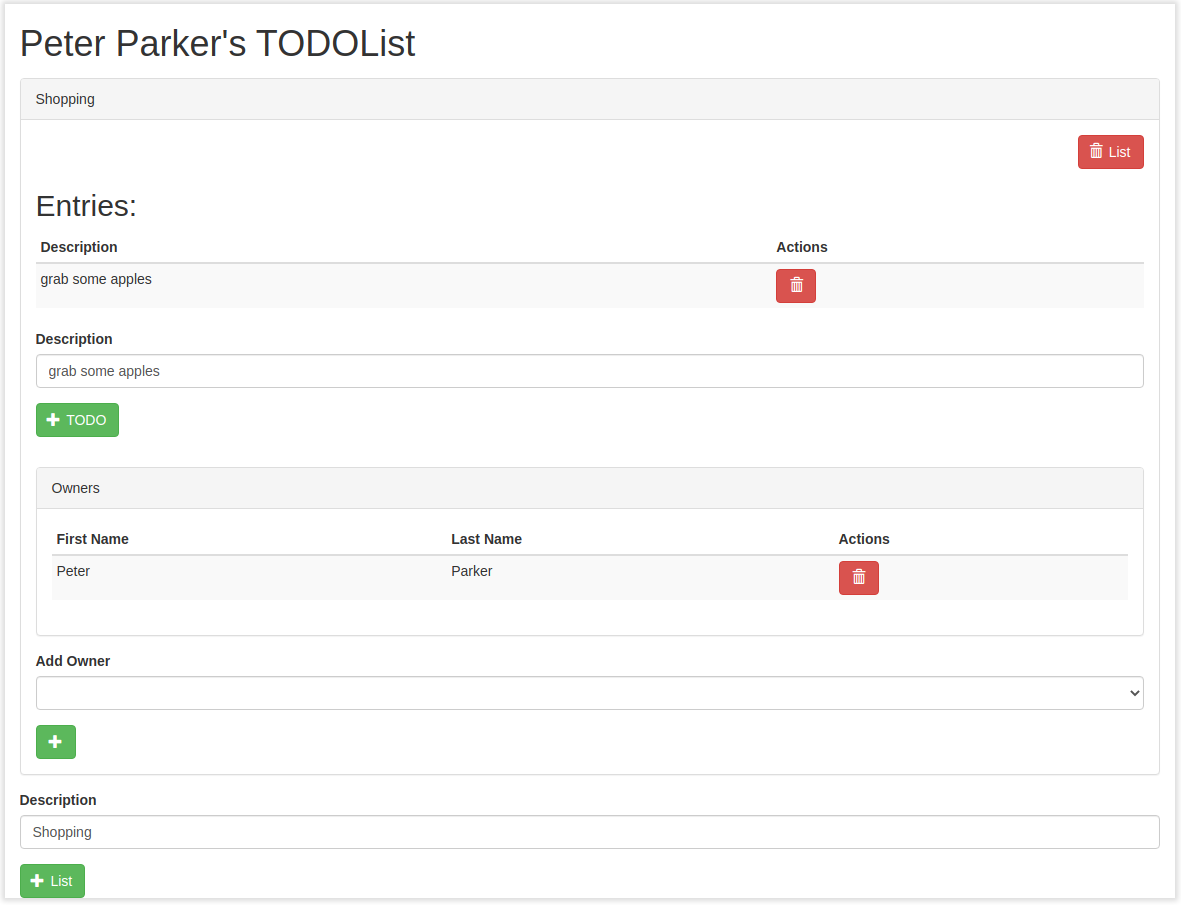
\includegraphics[width=0.8\textwidth]{todoApp.png}
    \caption{Impression of the TODO-App Web interface}
    \label{fig:todoApp}
\end{figure}

The TODO-App is an application that helps management lists of tasks that need to be done. It provides to a logged-in user with the possibility to create such lists, add various tasks to them, and after their completion, remove them~\cite{bosselmann-et_al}. Users also can add co-owners, which are other existing users, that can manage that respective list with them. The application is launched in development mode, meaning that it is accessible via a local Web address (\lstinline{http://localhost:8080}) from the host it has been started in. The TODO-App is ideal for demonstration purposes, since it presents all the Web elements necessary to a Web application interface. Figure \ref{fig:todoApp} shows said interface with all the elements the user can interact with, i.e.~buttons, input fields, dropdown selectboxes, etc.

DIME's model-driven development concept was our starting point. That is, the graphical elements meta specification is focused on specifying elements that represent the graphical user interface (GUI) and those that implement processes. The latter are elements whose semantic implementation will direct the Web browser to recreate the procedures necessary to construct the intended documentation. However, we should point out that in our scenario, the concept of data permanence is not required. Furthermore, even though our concept is based on DIME, it does not mean that our application is only for DIME-generated Web apps. In this respect, any navigable Web application can be modeled with our editor and thus documented.